% Bab 2: User Experience Scenario
\chapter{User Experience Scenario}
\label{bab:user-experience-scenario}
\section{Main Exploration Scenario}

\begin{longtable}{|L{0.500}|L{0.500}|}
\caption{Main Exploration Scenario}\\
\hline
\cellcolor[HTML]{D9EAF7}\textbf{{Aksi Aktor}} & \cellcolor[HTML]{D9EAF7}\textbf{{Reaksi Sistem}} \\ \hline
\endfirsthead
\hline
\cellcolor[HTML]{D9EAF7}\textbf{{Aksi Aktor}} & \cellcolor[HTML]{D9EAF7}\textbf{{Reaksi Sistem}} \\ \hline
\endhead
\multicolumn{2}{|L{1.000}|}{\textbf{Skenario Normal: Pengguna pertama kali memakai aplikasi, menjalankan Culinary Trail, lalu mencari tenant tambahan}} \\ \hline
Membuka aplikasi Mangan Yuk! untuk pertama kali &  \\ \hline
 & Menampilkan halaman login dengan tautan ke halaman registrasi \\ \hline
Mendaftar dengan nama pengguna, email, dan kata sandi &  \\ \hline
 & Menampilkan halaman onboarding (pengenalan aplikasi: jelajah kuliner, cerita budaya, culinary trail) \\ \hline
Menekan tombol Lanjut &  \\ \hline
 & Menampilkan penjelasan penggunaan lokasi (alasan, kapan lokasi dibaca, riwayat lokasi tidak dikirim ke server aplikasi, koordinat hanya dipakai layanan rute saat navigasi) dan tombol ``Izinkan Lokasi'' \\ \hline
Menekan tombol Izinkan Lokasi, lalu memilih ``Izinkan'' pada dialog sistem &  \\ \hline
 & Meminta izin notifikasi \\ \hline
Mengizinkan notifikasi &  \\ \hline
 & Meminta preferensi rasa (pedas/manis/gurih) dan jenis kuliner (makanan/minuman/jajanan), dengan opsi Lewati \\ \hline
Memilih preferensi pedas dan gurih, lalu menekan tombol Mulai &  \\ \hline
 & Menyimpan preferensi secara lokal, menampilkan Beranda (peta OSM + denah kawasan, posisi pengguna, status ``Di luar area'', jarak ke Sudirman Street Food, tombol Buka di Google Maps, Rencanakan Trail, dan Mode Jelajah) \\ \hline
Menekan tombol Buka di Google Maps &  \\ \hline
 & Membuka Google Maps dengan tujuan koordinat kawasan Sudirman Street Food \\ \hline
Menuju kawasan, kembali ke aplikasi, lalu mengaktifkan Mode Jelajah &  \\ \hline
 & Mengaktifkan pelacakan lokasi di background dan menampilkan notifikasi permanen ``Mangan Yuk! sedang memandu'' \\ \hline
Memasuki radius 100 m kawasan &  \\ \hline
 & Entry event: menampilkan notifikasi dan audio sambutan (``Selamat datang di Sudirman Street Food!''), menawarkan pilihan Rencanakan Trail atau Jelajah Bebas \\ \hline
Menekan notifikasi, lalu memilih Rencanakan Trail &  \\ \hline
 & Menampilkan form trail: durasi, budget, dan preferensi rasa (terisi otomatis dari onboarding) \\ \hline
Memilih durasi 60 menit, budget Rp50.000, lalu menekan tombol Buat Trail &  \\ \hline
 & Menampilkan itinerary 3 tenant berurutan beserta estimasi total biaya, estimasi waktu, dan rute di peta \\ \hline
Menekan tombol Mulai Trail &  \\ \hline
 & Menetapkan tenant pertama sebagai tujuan dan masuk mode navigasi (rute jalan kaki ke tujuan, jarak dalam meter, panah kompas), disertai audio ``Tenant pertama, 60 meter di depan'' \\ \hline
Memasukkan HP ke saku dan berjalan mengikuti arahan audio &  \\ \hline
 & Memberi panduan audio setiap jarak berkurang 20 m \\ \hline
Memasuki radius 25 m tenant pertama &  \\ \hline
 & Proximity event: HP bergetar dan memutar prompt ``Kamu mendekati [nama tenant]. Mau dengar ceritanya?'', notifikasi menampilkan tombol Dengar / Lewati \\ \hline
Menekan tombol Dengar dari lock screen &  \\ \hline
 & Memutar audio narasi cerita kuliner (asal-usul makanan, istilah Sunda, keunikan tenant) \\ \hline
Tiba dalam jarak \(\le\)10 m dari tenant &  \\ \hline
 & Memutar pengumuman ``Kamu sudah sampai!'' dan membuka kartu POI lengkap (foto, menu dan harga, cerita budaya, transkrip audio) \\ \hline
Memesan dan berada di tenant selama \(\ge\)3 menit &  \\ \hline
 & Dwell event: mencatat kunjungan secara otomatis dan menandai tenant pertama selesai pada trail \\ \hline
Masih makan di tenant melebihi alokasi waktu &  \\ \hline
 & Dwell event: mengirim notifikasi ``Sisa waktumu 30 menit, masih ada 2 tenant'' \\ \hline
Selesai makan dan berjalan keluar dari area tenant &  \\ \hline
 & Exit event: menampilkan tenant berikutnya beserta alasannya (misalnya ``30 m dari sini \(\cdot\) cocok setelah makanan pedas''), lalu masuk mode navigasi \\ \hline
Mengulangi alur navigasi, trigger, dan kunjungan untuk tenant kedua dan ketiga &  \\ \hline
 & Menjalankan trigger, memutar narasi, dan mencatat kunjungan otomatis untuk setiap tenant \\ \hline
Kunjungan di tenant terakhir selesai (dwell tercatat) &  \\ \hline
 & Menampilkan ringkasan trail (jumlah tenant, estimasi total belanja, durasi, dan jarak berjalan) \\ \hline
Menekan kolom pencarian dan mengetik ``batagr'' &  \\ \hline
 & Menampilkan hasil tenant batagor (toleran typo), diurutkan berdasarkan jarak \\ \hline
Memilih filter harga \textless{}Rp15rb, lalu memilih salah satu tenant &  \\ \hline
 & Menampilkan detail tenant dan tombol Jadikan Tujuan \\ \hline
Menekan tombol Jadikan Tujuan &  \\ \hline
 & Masuk mode navigasi menuju tenant yang dipilih \\ \hline
Tiba dalam jarak \(\le\)10 m dari tenant &  \\ \hline
 & Memutar pengumuman ``Kamu sudah sampai!'', membuka kartu POI, lalu mencatat kunjungan setelah pengguna berada \(\ge\)3 menit \\ \hline
Menekan tombol Selesai Jelajah &  \\ \hline
 & Mematikan pelacakan background, menghapus notifikasi permanen, dan kembali ke Beranda \\ \hline
\multicolumn{2}{|L{1.000}|}{\textbf{Skenario Alternatif 1: Pengguna menolak izin lokasi}} \\ \hline
Menekan ``Tolak'' pada dialog izin lokasi &  \\ \hline
 & Menampilkan penjelasan bahwa trigger otomatis dan navigasi tidak tersedia, dengan tombol Buka Pengaturan dan Lanjut tanpa Lokasi \\ \hline
Menekan tombol Lanjut tanpa Lokasi &  \\ \hline
 & Menampilkan peta tanpa posisi pengguna dan daftar tenant \\ \hline
Mengetuk salah satu tenant pada peta atau daftar &  \\ \hline
 & Menampilkan kartu POI dan tombol putar audio narasi (tanpa trigger otomatis dan navigasi) \\ \hline
\multicolumn{2}{|L{1.000}|}{\textbf{Skenario Alternatif 2: Pengguna memilih Jelajah Bebas}} \\ \hline
Memilih Jelajah Bebas pada notifikasi entry event &  \\ \hline
 & Menampilkan peta dengan seluruh marker tenant tanpa tujuan tertentu \\ \hline
Berkeliling kawasan tanpa tujuan &  \\ \hline
 & Memicu proximity event setiap kali pengguna mendekati tenant \\ \hline
Berhenti di tenant yang menarik \(\ge\)3 menit, lalu berjalan pergi &  \\ \hline
 & Mencatat kunjungan (dwell event), lalu saat exit event menampilkan 3 rekomendasi tenant berikutnya beserta alasannya \\ \hline
\multicolumn{2}{|L{1.000}|}{\textbf{Skenario Alternatif 3: Sinyal GPS lemah}} \\ \hline
Berjalan di area dengan sinyal GPS lemah (akurasi \textgreater{}30 m) &  \\ \hline
 & Mengabaikan pembacaan lokasi tersebut agar tidak terjadi trigger palsu, dan menampilkan banner ``Sinyal GPS lemah, trigger otomatis ditunda'' \\ \hline
Mengetuk daftar ``Tenant di sekitar'' atau marker tenant di peta &  \\ \hline
 & Menampilkan kartu POI dan audio narasi secara manual, lalu melanjutkan trigger otomatis setelah akurasi GPS kembali \(\le\)30 m \\ \hline
\multicolumn{2}{|L{1.000}|}{\textbf{Skenario Alternatif 4: Tenant pada trail tutup atau ingin dilewati}} \\ \hline
Menekan tombol Lewati Tenant pada mode navigasi &  \\ \hline
 & Menyusun ulang trail dengan tenant pengganti yang sedang buka, sesuai sisa waktu dan sisa budget, lalu menampilkan rute baru \\ \hline
\multicolumn{2}{|L{1.000}|}{\textbf{Skenario Alternatif 5: Pengguna menolak cerita saat proximity event}} \\ \hline
Menekan tombol Lewati pada notifikasi trigger &  \\ \hline
 & Menutup prompt audio, menyimpan tenant ke daftar ``Terlewati'', dan tidak memicu ulang tenant tersebut selama cooldown 30 menit \\ \hline
\multicolumn{2}{|L{1.000}|}{\textbf{Skenario Alternatif 6 (Optional): Pengguna mengumpulkan stempel Paspor Kuliner}} \\ \hline
Membuka menu Paspor Kuliner di Beranda &  \\ \hline
 & Menampilkan daftar trail tematik (misalnya ``Jejak Jajanan Sunda'' dan ``Manis-manis Bandung'') beserta progres masing-masing (misalnya 0/5) \\ \hline
Memilih trail ``Jejak Jajanan Sunda'' &  \\ \hline
 & Menampilkan daftar tenant yang termasuk trail tersebut dan menandainya di peta \\ \hline
Mengunjungi salah satu tenant pada trail dan berada di sana \(\ge\)3 menit &  \\ \hline
 & Dwell event: mencatat stempel digital untuk tenant tersebut, memutar efek suara singkat, dan memperbarui progres (1/5) \\ \hline
Mengunjungi tenant yang sama untuk kedua kalinya &  \\ \hline
 & Tidak mencatat stempel ganda; progres tetap 1/5 \\ \hline
Menutup aplikasi, lalu membukanya kembali di hari lain &  \\ \hline
 & Menampilkan progres paspor yang tersimpan (1/5) \\ \hline
Mengunjungi seluruh tenant pada trail hingga dwell tenant terakhir tercatat &  \\ \hline
 & Menampilkan badge ``Jejak Jajanan Sunda'' beserta audio ucapan selamat, dan menyimpan badge ke halaman Paspor Kuliner \\ \hline
\end{longtable}

\section{Main User Flow}

\begin{figure}[H]
\centering
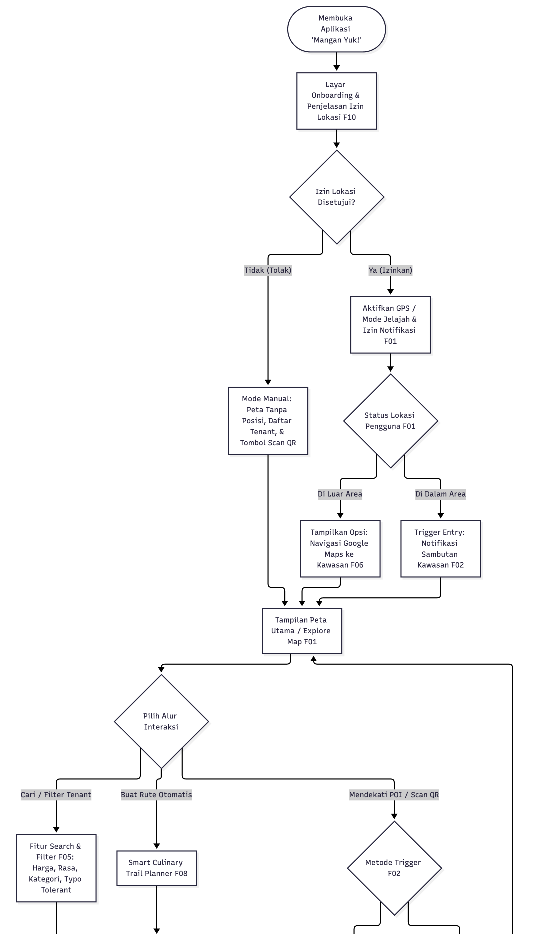
\includegraphics[width=0.9\textwidth,height=0.85\textheight,keepaspectratio]{images/user-flow-1.png}
\caption{Main User Flow aplikasi Mangan Yuk! (bagian 1 dari 3)}
\label{fig:user-flow-1}
\end{figure}

\begin{figure}[H]
\centering
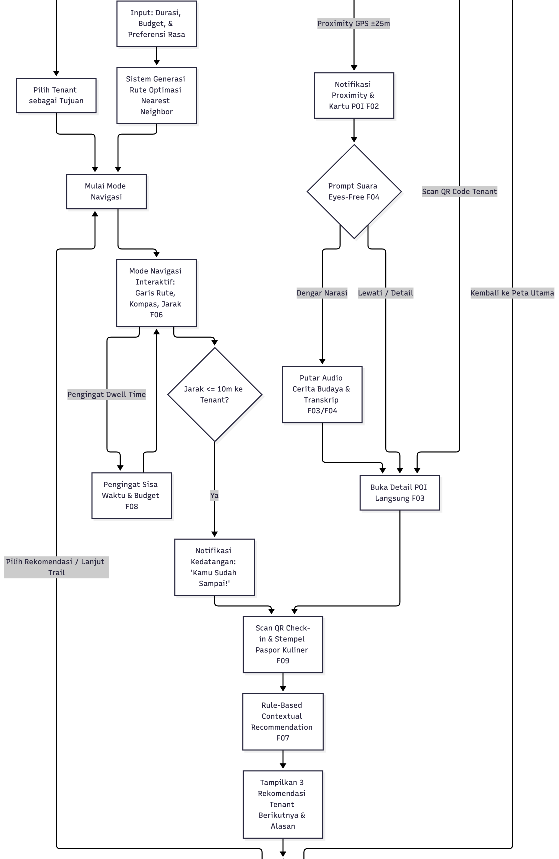
\includegraphics[width=0.9\textwidth,height=0.85\textheight,keepaspectratio]{images/user-flow-2.png}
\caption{Main User Flow aplikasi Mangan Yuk! (bagian 2 dari 3)}
\label{fig:user-flow-2}
\end{figure}

\begin{figure}[H]
\centering
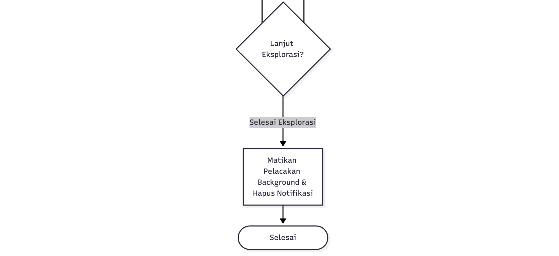
\includegraphics[width=0.9\textwidth,height=0.85\textheight,keepaspectratio]{images/user-flow-3.png}
\caption{Main User Flow aplikasi Mangan Yuk! (bagian 3 dari 3)}
\label{fig:user-flow-3}
\end{figure}
